\documentclass[handout]{beamer}
% L'option handout permet de supprimer la barre de navigation

\usepackage[T1]{fontenc}
\usepackage[utf8]{inputenc}
\usepackage[french]{babel}
% Pour utiliser le signe €
\usepackage{eurosym}
% Pour pouvoir insérer des images
\usepackage{graphicx}
\usepackage{wrapfig}
% Gestion des couleurs
\usepackage{color}
\definecolor{QTPurple}{RGB}{61, 68, 160} %3D44A0

\usepackage{hyperref}

% Un joli thème flat
\usetheme{Rochester}

% Personnalisation du thème
\usecolortheme[named=QTPurple]{structure}
\setbeamertemplate{blocks}[shadow=false]

% ------------------------------------ %
% -- METADONNÉES DU DOCUMENT --------- %
\title[Stats]{
	Statistiques pour l'ingénieur\\
	Validation croisée
}
\author{
	Étienne Batise - Thibaud Dauce
}
\date{\today}

% \titlegraphic{\includegraphics[height=.3\textheight]{images/logo.png}}

% Début du document
\begin{document}
	
	% Génération de la page de titre
	\begin{frame}[plain]
		\titlepage
	\end{frame}

	% Génération du sommaire
	\begin{frame}[plain]
		\frametitle{Sommaire}
		\tableofcontents
	\end{frame}


	% ///////////////////////////////////////////////////////// %
	% /// Qu'est-ce que la validation croisée ? /////////////// %
	\section{Qu'est-ce que la validation croisée ?}

	\subsection{L'utilité}
		\begin{frame}
		\frametitle{L'utilité}
		\begin{tabular}{l l}
			\begin{minipage}{0.2\textwidth}
				\begin{center}
					
\includegraphics[width=0.9\textwidth]{images/cross.png}
				\end{center}
			\end{minipage}

			\begin{minipage}{0.8\textwidth}
				\begin{itemize}
					\item tester les données...
					\item ...avec peu de points
					\item ...sans faire trop de calculs
				\end{itemize}
			\end{minipage}

		\end{tabular}
		\end{frame}

	\subsection{Le principe}
		\begin{frame}
		\frametitle{Le principe}
		\begin{tabular}{l l}
			\begin{minipage}{0.5\textwidth}
				\begin{center}
					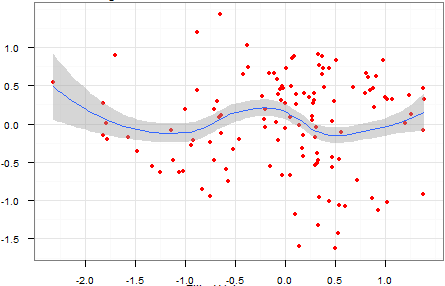
\includegraphics[width=0.8\textwidth]{images/function.png}
				\end{center}
			\end{minipage}

			\begin{minipage}{0.5\textwidth}
				\begin{itemize}
					\item après avoir trouvé la fonction
					\item tester sa validité
					\item deux groupes de données :
						\begin{itemize}
							\item groupe d'apprentissage
							\item groupe de test
						\end{itemize}
				\end{itemize}
			\end{minipage}
			
		\end{tabular}
		\end{frame}

	\subsection{3 types de validation croisée}
		\begin{frame}
		\frametitle{3 types de validation croisée}
		\begin{tabular}{l l}
			\begin{minipage}{0.2\textwidth}
				\begin{center}
					
\includegraphics[width=0.9\textwidth]{images/clock.png}
				\end{center}
			\end{minipage}

			\begin{minipage}{0.8\textwidth}
				\begin{itemize}
					\item Rapport données / temps de calcul 
					\begin{itemize}
						\item testset validation
						\item leave-one-out cross-validation
						\item k-fold cross-validation
					\end{itemize}
				\end{itemize}
			\end{minipage}

		\end{tabular}
		\end{frame}

		\begin{frame}
		\frametitle{testset validation}
		\begin{tabular}{l l}
			\begin{minipage}{0.5\textwidth}
				\begin{center}
					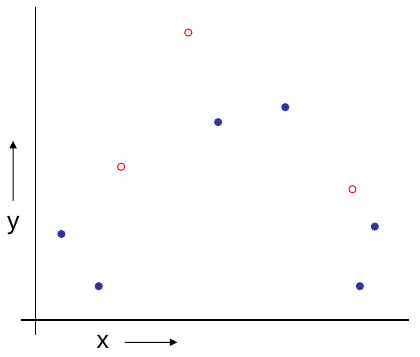
\includegraphics[width=0.9\textwidth]{images/testset.png}
				\end{center}
			\end{minipage}

			\begin{minipage}{0.5\textwidth}
				\begin{itemize}
					\item choisir 30\% des données pour le test
					\item Résultats :
					\begin{itemize}
						\item très facile à mettre en place
						\item perte de 30\% de l'échantillon
						\item peu précis en cas de petit échantillon
					\end{itemize}
				\end{itemize}
			\end{minipage}

		\end{tabular}
		\end{frame}

		\begin{frame}
		\frametitle{leave-one-out cross-validation}
		\begin{tabular}{l l}
			\begin{minipage}{0.5\textwidth}
				\begin{center}
					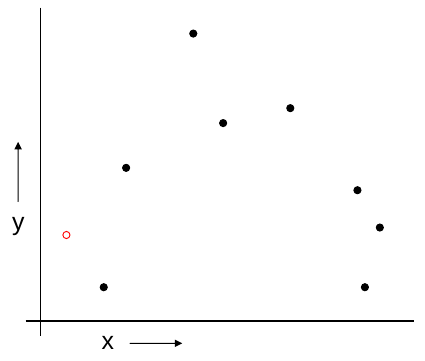
\includegraphics[width=0.9\textwidth]{images/leave-one-out.png}
				\end{center}
			\end{minipage}

			\begin{minipage}{0.5\textwidth}
				\begin{itemize}
					\item choisir 1 donnée pour le test
					\item recommencer pour chaque donnée
					\item faire la moyenne des erreurs
					\item Résultats :
					\begin{itemize}
						\item aucune perte de données
						\item très couteux en temps
					\end{itemize}
				\end{itemize}
			\end{minipage}

		\end{tabular}
		\end{frame}

		\begin{frame}
		\frametitle{k-fold cross-validation}
		\begin{tabular}{l l}
			\begin{minipage}{0.5\textwidth}
				\begin{center}
					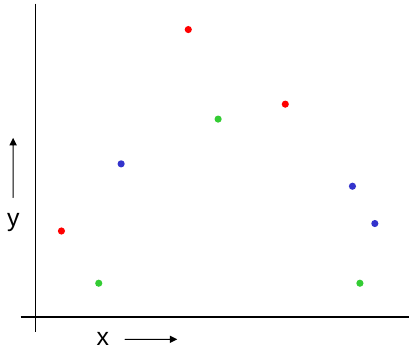
\includegraphics[width=0.9\textwidth]{images/k-fold.png}
				\end{center}
			\end{minipage}

			\begin{minipage}{0.5\textwidth}
				\begin{itemize}
					\item découper les données en k parties
					\item Résultats :
					\begin{itemize}
						\item perte de données relative à k
						\item complexité relative à k
						\item si k = n, équivalent à un leave-one-out
					\end{itemize}
				\end{itemize}
			\end{minipage}

		\end{tabular}
		\end{frame}

	% //////////////////////////////////////////// %
	% /// Démonstration Octave /////////////////// %
	\section{Démonstration Octave}

	\begin{frame}
	\frametitle{Présentation du code}
	\begin{tabular}{l l}
		\begin{minipage}{0.4\textwidth}
			\begin{center}
				
\includegraphics[width=0.9\textwidth]{images/octave.png}
			\end{center}
		\end{minipage}

		\begin{minipage}{0.6\textwidth}
			\begin{itemize}
				\item génération de points aléatoires
				\item calcul de la fonction par 2 méthodes : 
					\begin{itemize}
						\item régréssion linéaire
						\item régréssion quadratique
					\end{itemize}
				\item calcul de la validation croisée
			\end{itemize}
		\end{minipage}

	\end{tabular}
	\end{frame}

	% //////////////////////////////////////////// %
	% /// Et maintenant, dans l'informatique ///// %
	\section{Et maintenant, dans l'informatique}

	\subsection{Exemple des réseaux de neurones 1/2}
		\begin{frame}
		\frametitle{Exemple des réseaux de neurones 1/2}
		\begin{tabular}{l l}
			\begin{minipage}{0.4\textwidth}
				\begin{center}
					
\includegraphics[width=0.9\textwidth]{images/neural_networking.jpg}
				\end{center}
			\end{minipage}

			\begin{minipage}{0.6\textwidth}
				\begin{itemize}
					\item modèle de calcul basé sur les neurones biologiques
					\item une ou plusieurs entrées, une sortie
					\item fonctionne en couche
					\item permet de résoudre des problèmes statistiques
					\item basé sur l'apprentissage
				\end{itemize}
			\end{minipage}
			
		\end{tabular}
		\end{frame}

	\subsection{Exemple des réseaux de neurones 2/2}
		\begin{frame}
		\frametitle{Exemple des réseaux de neurones 2/2}
		\begin{tabular}{l l}
			\begin{minipage}{0.2\textwidth}
				\begin{center}
					
\includegraphics[width=0.9\textwidth]{images/ajust.png}
				\end{center}
			\end{minipage}

			\begin{minipage}{0.8\textwidth}
				\begin{itemize}
					\item tester son réseau de neurones
					\item ajuster l'apprentissage
					\begin{itemize}
						\item nombre de noeuds
						\item paramètres d'apprentissage
					\end{itemize}
					\item pour en savoir plus : cours "Machine Learning" sur Coursera
				\end{itemize}
			\end{minipage}
			
		\end{tabular}
		\end{frame}

	\section{Questions}
		\begin{frame}
		\frametitle{Questions}
		On vous écoute :)
		\vspace{40px}
		\tiny{
			\begin{itemize}
				\item \url{http://www.autonlab.org/tutorials/overfit10.pdf}
				\item \url{https://fr.wikipedia.org/wiki/Réseaux\_de\_neurones}
				\item \url{https://jamesmccaffrey.wordpress.com/2013/10/25/k-fold-cross-validation-for-neural-networks}
				\item \url{http://visualstudiomagazine.com/articles/2013/10/01/understanding-and-using-kfold.aspx}
				\item \url{https://fr.wikipedia.org/wiki/Validation\_croisée}
				\item \url{https://www.coursera.org/course/ml}
			\end{itemize}
		}
		\end{frame}

	% ///////////////////////////////////////////////////////// %

% Fin du document
\end{document}
